\documentclass[11pt,a4paper]{article}
\usepackage{ifpdf}
\usepackage[utf8]{inputenc} \usepackage[francais]{babel}
\usepackage[T1]{fontenc} \usepackage[nottoc, notlof, notlot]{tocbibind}
\usepackage[unicode=true,pdftex,colorlinks=true,linkcolor=black,urlcolor=black,citecolor=black]{hyperref}
\usepackage{natbib}
\usepackage{graphicx}
\usepackage{array}

\parindent 0.8cm
% \setlength{\parskip}{0.5em plus 0.2em minus 0.2em}

\title{Projet B: gestion de dossier}
\author{Anthony \textsc{Caillaud} Manoël \textsc{Fortun} Charles \textsc{Dejean}}
\date{\today}
\ifpdf \pdfinfo { /Author (Anthony Caillaud Manoël Fortun  
Charles Dejean) /Title (Projet B rapport) /Subject (Gestion de dossier) /Keywords ()
/CreationDate (D:20100329212218) } \fi


\begin{document}

\maketitle

\clearpage \tableofcontents \clearpage


\section{Introduction}

Ce rapport reprend notre travail dans le cadre de notre module de construction formelle de logiciel à l'aide de la méthode, ce rapport reprend donc notre travail sur le mini projet de ce module. Ce mini projet concernait une gestion générique de dossier, des dossiers
client pour une entreprise, de dossier médical pour des patients, donc quelque chose de générique.
Ce rapport reprend donc les différentes étapes de notre travail sur ce mini projet, partant de la phase d'analyse avec le cahier des charges. Puis la partie specification avec des diagrammes patates et définitions. Et ensuite la partie devellopement avec les machines B, le raffinement et finalement l'arrivé au code.

\section{Analyse}

\subsection{cahier des charges}

La gestion de dossier est un problème récurrent en informatique, pas de dossier dans le sens arboressence mais dossier informatisé
contenant des informations comme un dossier de patient d'hopital, dossier de client, etc. Quelque soit le domaine d'application il y a un certain nombre de point commun à ces gestions de dossier. Notre projet s'articule donc autour de cette problématique généraliste.

On dégage de celà les éléments générique de la gestion de dossier. Un dossier à un identifiant unique, une date de création, l'identifiant du créateur et une collection de modification liée à ce dossier. Le terme modification peut désigner beaucoup de chose, ici celà ne nous intéresse pas vraiment. Une modification possède une date, un identificateur de personne faisant la modification, un libellé, un état et un numéro permettant d'ordonner et d'identifier les modifications, puisque plusieurs modifications peuvent avoir la même date.

Le projet doit contenir un minimum pour la gestion d'employé, de façon très générique pour avoir au minimum des id d'employés nécessaire pour la gestion des dossiers tel qu'elle est décrite précédement. 


\subsection{Raffinement du cahier des charges}

Ici nous allons décrire de manière plus pratique les fonctionnalités et propriétés présentées dans le cahier des charges.

\subsubsection{Propriétés}

\begin{tabular}{|l|p{30em}|}
  \hline
  Propriété & Description \\
  \hline
  Employé & Un employé possède un id unique numérique, un nom, un prénom et un état \\
  \hline
Etat employé & Les états d'employés sont inactif ou actif  \\
  \hline
Dossier & Représentation d'un dossier comprenant: un id numérique unique, date de création, Id employé créateur et  une collection de modification  \\
  \hline
Modification & Une modification possède un id numérique correspondant à l'ordre de création des modifications pour ce dossier, une date, un id d'employé créateur de la modification, un état de traitement et un libellé de traitement  \\
  \hline

Etat de traitement & Un dossier peut avoir comme état: Pret, attente ou fermé  \\
  \hline
Libellé de traitement &  Le libellé de traitement est une chaine de caractère prise dans un ensemble prédéfini dépendant du contexte d'utilisation\\
  \hline


\end{tabular}




\subsubsection{Fonctionnalités}

On va distinguer trois types fonctionnalités, d'abord les fonctionnalités pour les dossiers:

\begin{tabular}{|l|p{30em}|}
  \hline
  Fonctionnalités & Description \\
  \hline
  Créer dossier & Permet de créer un dossier prend en paramètre l'id de l'employé et la date du jour, on retourne l'id du nouveau dossier \\
  \hline
Modifier Etat Traitement &   Permet de modifier l'état de traitement d'un dossier, prend en paramètre l'id du dossier, le numéro de la modification et le nouvel état\\
  \hline
Tracer Opération & Permet de créer une nouvelle modification avec en paramètre date, l'id employé, l'id du dossier et un libellé de traitement \\
  \hline
Supprimer Dossier & Supprime un dossier et toutes les modifications liées, il faut donner l'id du dossier et celui du créateur du dit dossier\\
  \hline

\end{tabular}\\


Puis celle pour les employés:


\begin{tabular}{|l|p{30em}|}
  \hline
  Fonctionnalités & Description \\
  \hline
  Creer Employé & Créer un employé, il faut en paramètre son nom et prénom, en sortie on lui attribut automatiquement un id et l'état actif \\
  \hline
Modifier Etat Employé &   En entré on donne l'id et le nouvel état \\
  \hline
Supprimer Employé & On supprime l'employé avec en entré son id, mais on conserve l'id dans les id utilisés pour conserver les traces de ses modifications. \\
  \hline

\end{tabular}\\

Et enfin celle pour l'affichage, sélection:

\begin{tabular}{|l|p{30em}|}
  \hline
  Fonctionnalités & Description \\
  \hline
  roquettes & \\
  \hline
roquettes &   \\
  \hline
roquettes & \\
  \hline

\end{tabular}\\


\subsection{Organisation du temps de travail}

 On pourra voir en figure \ref{diagant}  l'organisation de notre travail représenté avec un diagramme de gant.


\begin{figure}[h]
  	%[height=12cm,width=15cm]
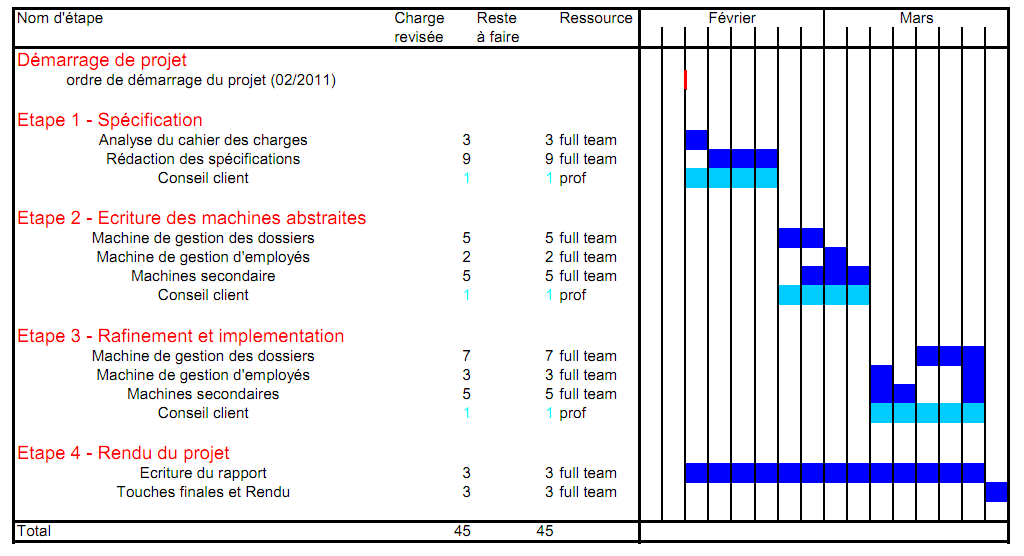
\includegraphics[height=12cm,width=17cm]{diaGant.png}
  		\caption{Diagramme de gant}
  		\label{diagant}
\end{figure}



\section{Specification}

\subsection{Diagramme de pattate}

\begin{figure}[h]
  	%[height=12cm,width=15cm]
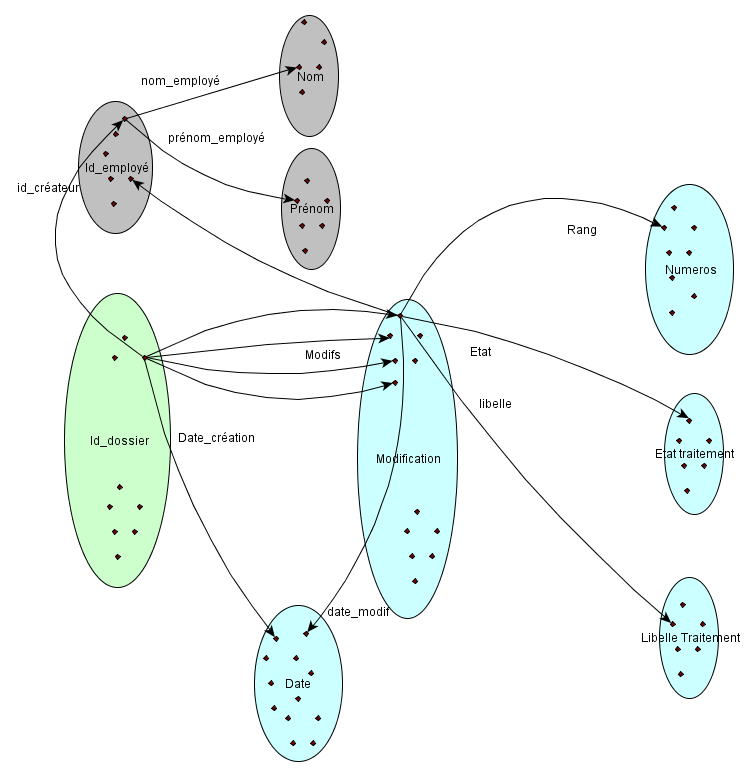
\includegraphics[height=12cm,width=17cm]{pattate.png}
  		\caption{Diagramme de pattate}
  		\label{pattate}
\end{figure}


\subsection{Définitions des relations}




\subsection{Architecture des machines}


\subsection{Plan de raffinage}


\section{Développement}

\subsection{raffinage}


\subsection{l'implémentation}


\subsection{le code}



\section{conclusion}

Plus de temps que d'habitude, 



%
%\begin{figure}[h]
  	
%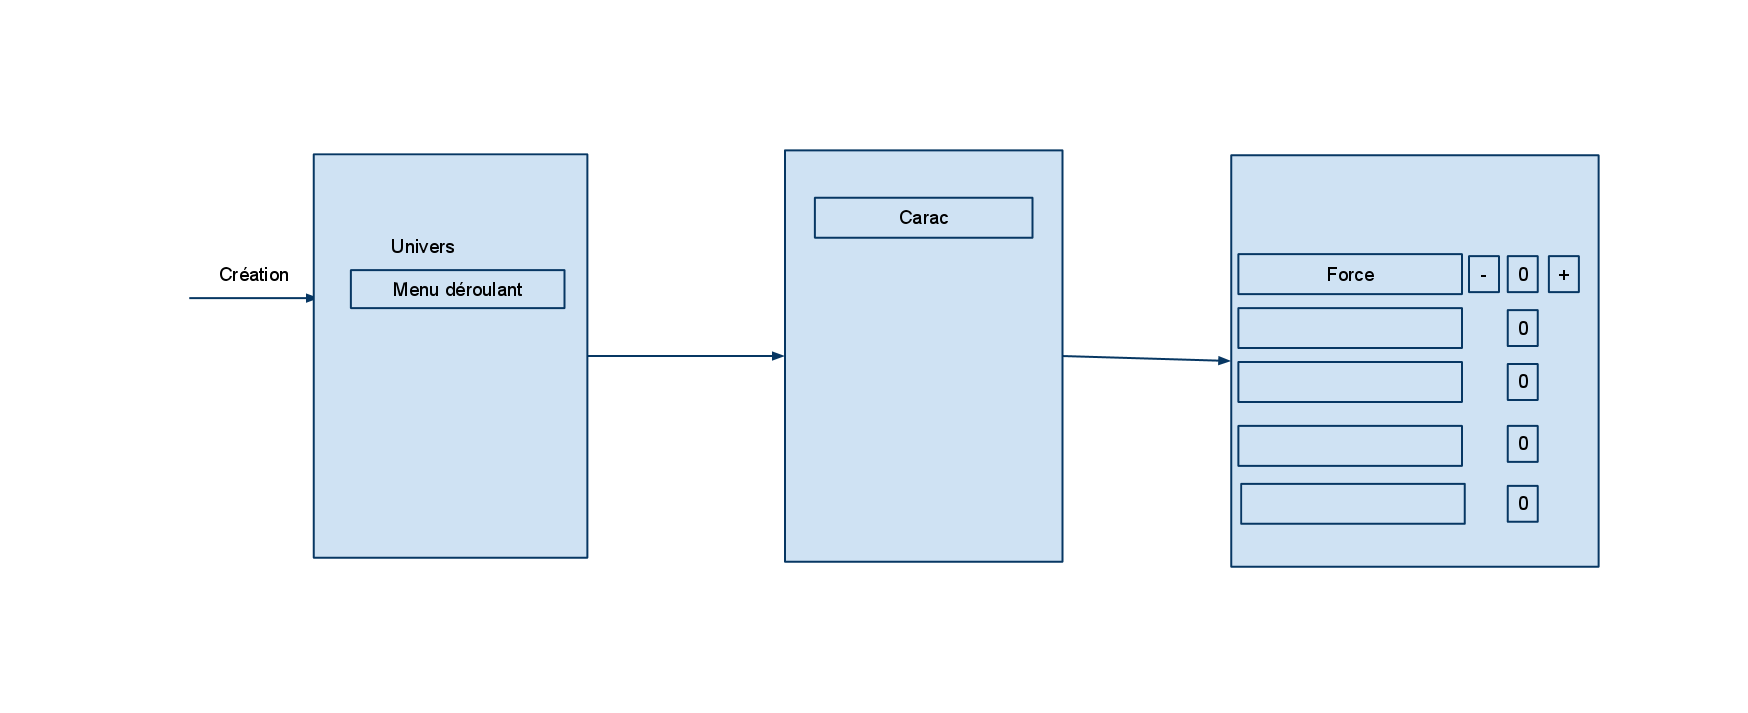
\includegraphics[height=12cm,width=15cm]{image/screen5.png}
  	%	\caption{Création de personnage}
  	%	\label{screen5}
%\end{figure}

% \ref{screen5} 


%\begin{itemize}
%  \item DiceModule : il fournit différentes méthodes permettant d'effectuer
% plusieurs types de jet de dés.
%  \item FicheModule : il permet d'enregistrer/charger une fiche de personnage à
%  partir d'un modèle de fiche ou bien à partir d'une fiche même. Cela comprend
%  aussi le parseur xml nécessaire à ces opérations.
% \item SystemModule : idem que FicheModule mais pour un système de règles.
%\end{itemize}

%\begin{tabular}{|l|c|r|}
 % \hline
 % colonne 1 & colonne 2 & colonne 3 \\
 % \hline
%1.1 & 1.2 & 1.3 \\
 % 2.1 & 2.2 & 2.3 \\
%  \hline
%\end{tabular}

\end{document}